\documentclass[10pt]{article}
\usepackage{grafematik}

\title{Malayalam Orthographic Reforms: \\Impact on Language and Popular Culture}

\author{Kavya Manohar \\
\small{Swathanthra Malayalam Computing} \\
 {\small {\tt sakhi.kavya@gmail.com}} \\
 \and
 Santhosh Thottingal \\
 \small{Swathanthra Malayalam Computing} \\
 {\small {\tt santhosh.thottingal@gmail.com}}}

%\date

%\date{October 2017}

\begin{document}

\maketitle

\begin{abstract}

Malayalam is a language spoken in India, predominantly in the state of Kerala with about 38 million native speakers. The Malayalam script evolved from Brahmi through Grantha lipi and Vattezhuthu writing systems. The script orthography has acquired its uniqueness with it's complex shaped graphemes formed by the combination of consonant sequences and signed vowel forms. The number of unique graphemes in this system exceeds fifteen hundred. The orthographic styles were constantly evolving. In 1971 there was a Governmental intervention in the orthograhy, to reduce its complexity to minimise the labour on typesetting and printing. This paper is an attempt to bring out the impact of this orthographic reforms on various aspects of script usage including popular culture, media, textbooks, graffiti and handwriting. It will also analyse the impact of Unicode and the advancement in digital typography on the orthographic diversity of Malayalam script.

\end{abstract}
 \textbf{Keywords:} Malayalam Script, Orthography Reforms, Unicode, Graphemes, Media and Communication, Digital Typography

\section{Introduction}

\paragraph{}

With 38 million native speakers Malayalam is the official language of Kerala, India. Malayalam used to be written in Vattezhuthu, a script for Tamil, another south Indian language. The modern Malayalam script evolved from Grantha alphabet which was a script for Sanskrit. Both Vattezhuthu and Grantha has its roots in the Brahmi script\footnote{Malayalam Script in English Wikipedia: \url{https://en.wikipedia.org/wiki/Malayalam_script}}. The modern Malayalam script has 15 vowels and 36 consonants as the basic character set. The vowels have signed notations to be used with consonants.

\paragraph{}
The script is mainly abugida, or alphasyllabary. That is, consonant–vowel sequences are written as a unit: each unit is based on a consonant or conjunct letter, and vowel notation is secondary. Vowels have independent existence, but only at word beginnings. This is the common characterestic of Brahmic family of scripts of South and Southeast Asia.

\section{Script and the nature of graphemes}

\paragraph{}
The script has acquired its uniqueness with it's complex shaped ligatures formed by the consonants and conjuncts with signed vowel forms. Conjuncts are formed by a sequence of two more consonants. The conjunct grapheme usually has a shape smoothly blend from the constituent consonants. The Figure \ref{mathan} illustrates one of the earliest books printed in Malayalam script, A Grammar of Malayalim, by Rev. George Mathan and printed in 1863 \cite{georgemathan}. The cited page tabulates the vowels and their signed notations with consonants. 

\begin{figure}[h!]
	\centering
	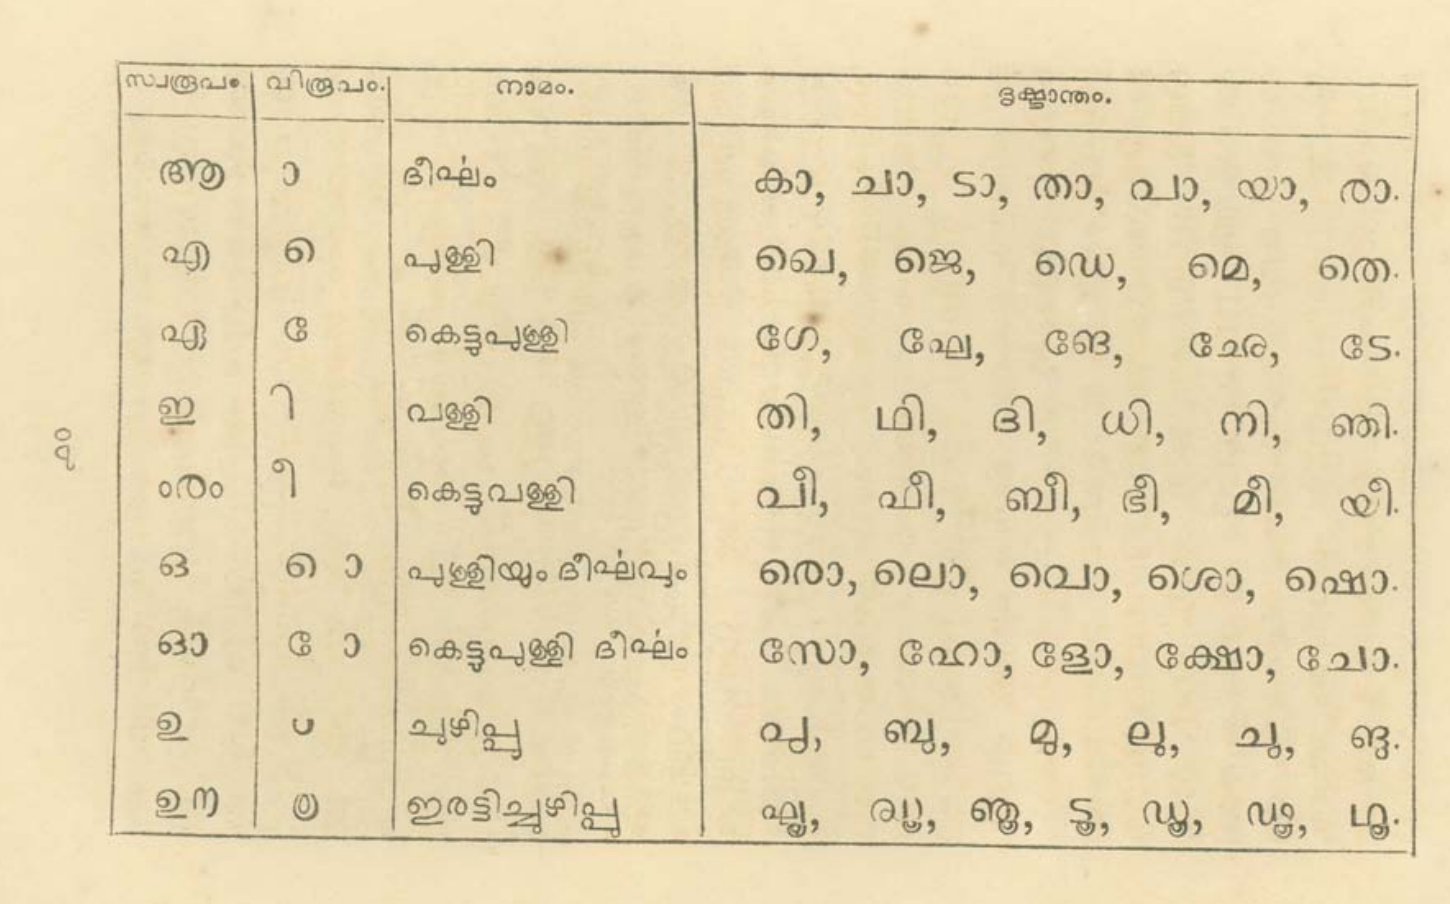
\includegraphics[width=0.8\textwidth]{images/mathanSymbols.png}
	\caption{A Grammar of Malayalam(1863)}
	\label{mathan}
\end{figure} 

The characteristics of the graphemes of Malayalam script are listed below:

\begin{itemize}
\item
Vowels and consonants are the basic building blocks of Malayalam script. 
\item
 Vowels have stand alone existence in their pure form. Vowels in Malayalam: {\manjari അ, ഇ, എ }
\item
Alternately vowels also appear as signed form modifying a consonant sound, vowel signs have no existance without a consonant. Vowel signs in Malayalam: {\manjari ി, ീ}
\item Consonants in Malayalam always have the inherent vowel /a/ present in them. Consonants in Malayalam: {\manjari ക, ത, ഗ, ദ, ധ }
\item
 Any other vowels sound associated with a consonant is written as a signed form of the consonant. The signs can be prebase, postbase or both. Some signs modify the shape of base grapheme. Consonants with vowel signs:  {\manjari കി, ഗു, ധെ } 

\item
The removal of inherent /a/ in a consonant is marked in the script by a special character \textit{virama}. Consonant with virama sign: {\manjari ക് }
\item
Virama after a consonant not only removes inherent /a/ but also indicate no vowel sound follows it. 
\item
A conjunct is formed by  a sequence of consonants with no vowel sound in between. In other words , consonants separated by virama forms a consonant. Conjuncts: {\manjari ക+്+ത -> ക്ത , ഗ+്+ദ ->ഗ്ദ }
\item
 A conjunct can also be formed by a consonant which follows another conjunct with no vowelsign in between. That is a conjunct followed by a virama and a consonant forms a new conjunct. Every conjunct can be modified by a vowel sign. {\manjari ഗ്ദ+്+ധ ->ഗ്ദ്ധ, ഗ്ദ്ധ+ു -> ഗ്ദ്ധു }

\item
Some consonats involved in the formation of conjuncts have signed forms. eg:{\manjari{ ്‌ര, ്‌ല, ്‌യ, ്‌വ, ര് . ക+്‌ര -> ക്ര, ക+്‌ല ->ക്ല , ക+്‌യ -> ക്യ, ക്+്‌വ -> ക്വ, ര്+ക-> ൎക}}
 
\item 
Certain consonants have a unique grapheme represenatation in their pure form named \textit{chillu}. {\manjari ൿ, ൾ, ൺ, ൻ, ൽ, ർ }
\end{itemize}


\paragraph{}

 The Orthographic styles were continuously evolving. The shapes of conjuncts, relative positioning of signs and their sizes have changed over time to match the needs of writing schemes. Stylus on dry palm leaves gave limited flexibility and the graphemes were rarely perfect rounds. But pen on paper made it more curvy. 

\section{Script in Early Prints }

\paragraph{}
The first ever book in Malayalam script was printed in Rome, in 1772. Printing in Malayalam started natively during 1820s\cite{babucherian}. When printing technology started getting popular there was a requirement to cast movable types in huge numbers. Even though the basic characters were less than hundred, the orthographic style demanded separate types for conjuncts, and their signed vowel forms. Apart from vowels, some consonants too have signed notations, further increasing the number of types needed in the foundry. 

\subsection{Historic Evolution}

\paragraph{}
The first printed book in Malayalam using movable types, {\manjari സംക്ഷെപവെദാർത്ഥം} (Samkshepavedartham) in 1772 had more than thousand unique types\cite{babucherian}. The manual labour on typesetting and lay outing were high for the same reason. 

\begin{wrapfigure}{L}{0.6\textwidth}
 \centering
  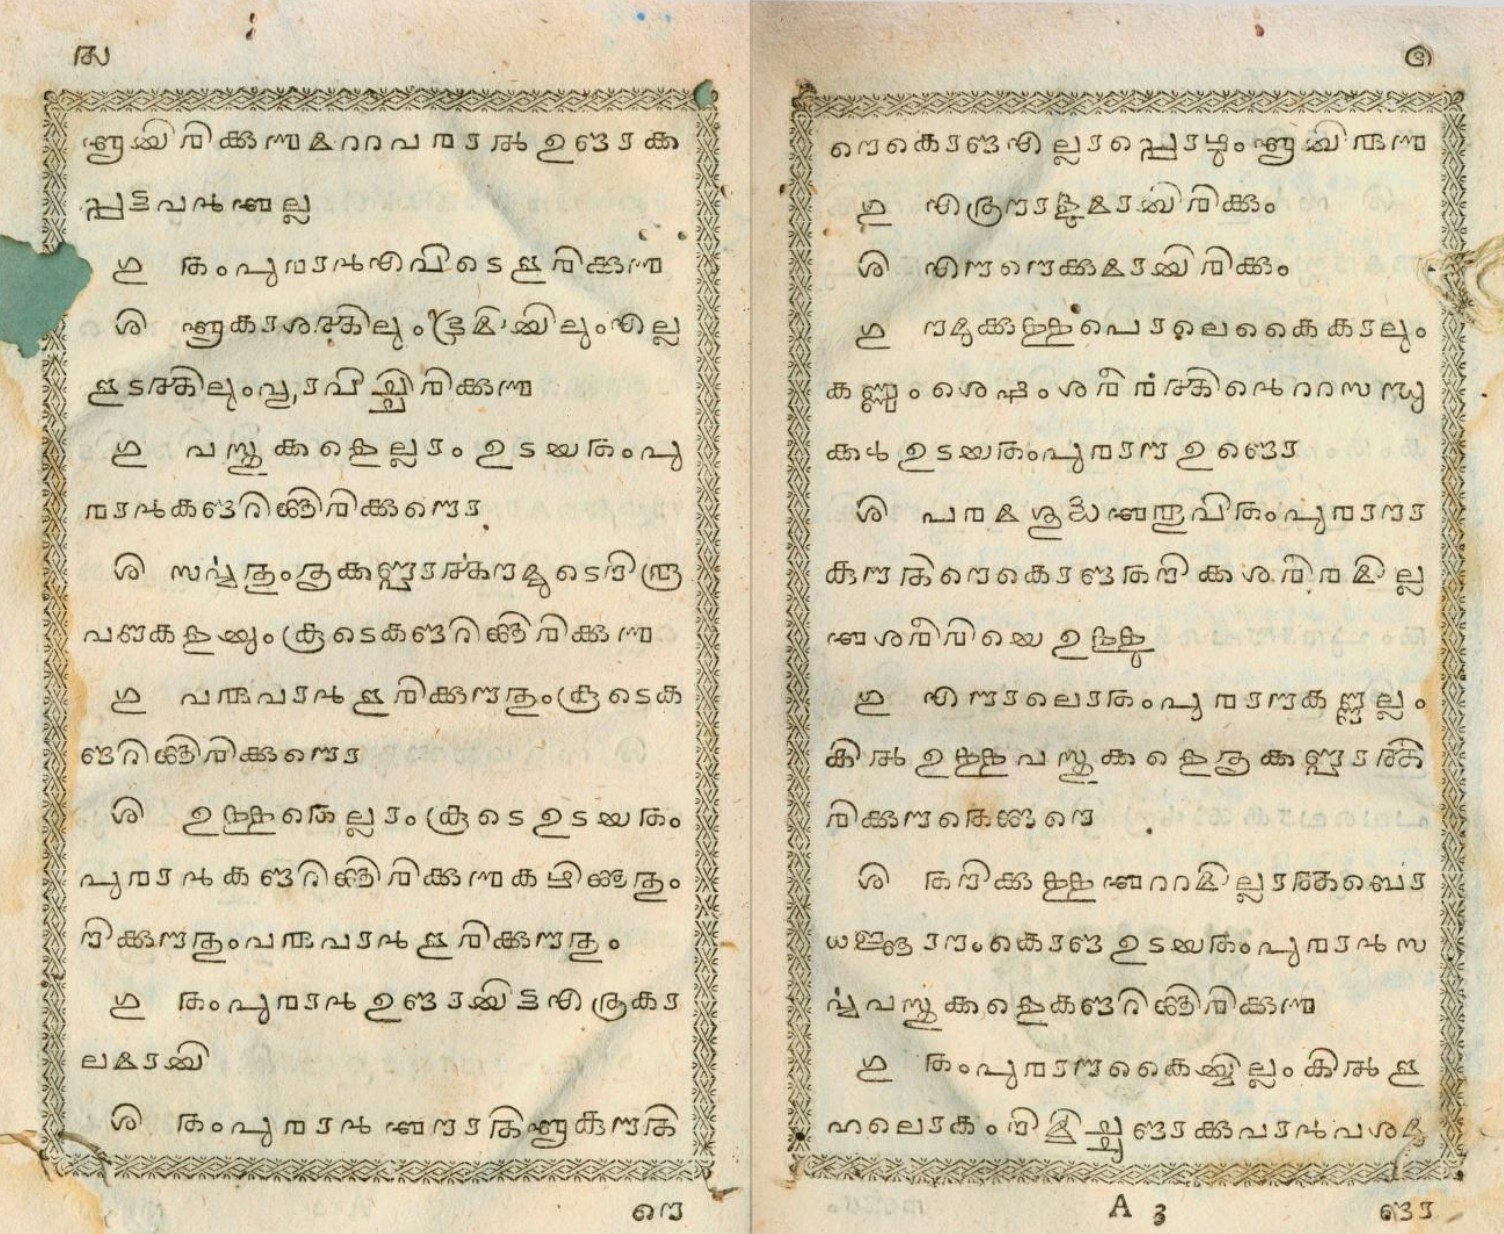
\includegraphics[width=0.55\textwidth]{images/samkshepavedartham1772.png}
   \caption{Samkshepavedartham (1772)}
	\label{Samkshepam}
\end{wrapfigure}

\paragraph{}
Figure \ref{Samkshepam} shows pages from the catechism book Samkshepavedartham. The script is mostly rectangular. The types were made and printing was done in Rome. The first native type casting and printing was done by Benchamin Bailey, an Anglican missionary in 1829.  His contributions as a typographer made the curvy style of the Malyalam orthography popular\cite{gupthannair}.


\paragraph{}
The Figure \ref{newtestament}, shows pages from The New Testament printed using the types designed by Benchamin Bailey, imprinted in 1829\cite{babucherian}. The script continued to evolve by separating some vowel sign types ({\manjari{  ി, ീ } }) from the consonant/conjunct grapheme. Still the richness of conjuncts and their signed forms were largely retained. It can be seen from Figure \ref{Sabdatharavali}. 


\begin{figure}[h!]
\begin{subfigure}{.5\textwidth}
 \centering
 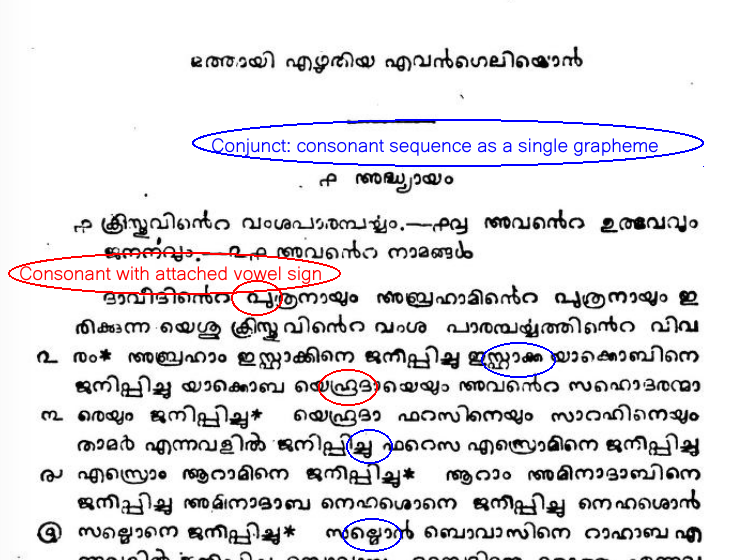
\includegraphics[width=\linewidth, height=5cm]{images/newtestament1829.png}
 \caption{New Testament (1829)}
 \label{newtestament}
\end{subfigure}%
\begin{subfigure}{.5\textwidth}
 \centering
 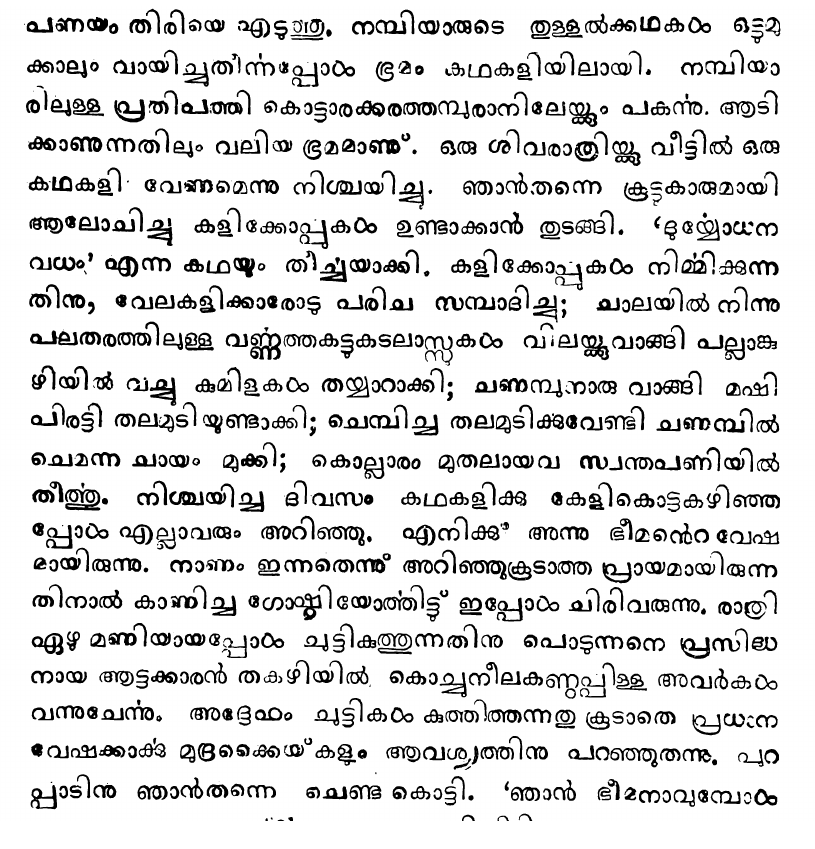
\includegraphics[width=\linewidth,height=5cm]{images/1930-Sabdatharavali.png}
 \caption{Sabdatharavali(1930)}
 \label{Sabdatharavali}
\end{subfigure}
\caption{Comparing the Malayalam scripts in print}
\end{figure}


\section{Reformation}

\paragraph{}
In 1971, there was a governmental order by the state of Kerala intended to reduce the complexity of the script. The proposal was to discard the usage of complex conjuncts and to separate the vowel notations from the consonants and conjuncts. The orthography reformation proposal was to reduce the challenges imposed by the script on the typesetting and printing technology. Being a forced intervention, this was a major event to be marked in the history of the orthographic evolution. 

\begin{figure}[h!]
 \centering
  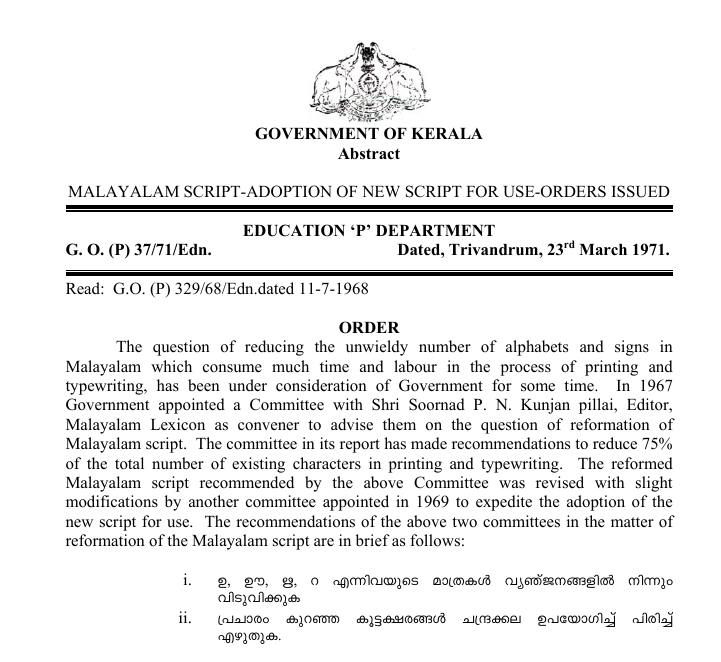
\includegraphics[width=0.8\textwidth]{images/1971-gov-script-reformation-order.png}
   \caption{The Government Order on Malayalam Script Reform in 1971}
	\label{go1971}
\end{figure}

Figure \ref{go1971} shows the front page of government order proposing the new orthography style. The proposal aimed at reducing the grapheme usage in Malayalam by 75 percentage. The major proposals in the order are following:\cite{1971go}

\begin{itemize}
\item
Detatch the signs of vowels {\manjari ഉ, ഊ and ഋ } from the base grapheme.\\
{\manjari കു } -> {\raghu കു } ,
{\manjari കൂ } -> {\raghu കൂ } ,
{\manjari കൃ } -> {\raghu കൃ } .

\item 
Detatch the consonat sign {\manjari  ്ര } from the base grapheme \\
{\manjari ക്ര  } -> {\raghu ക്ര  } 

\item
Discard the usage of {\manjari ര് } in the consonant sequence in signed form as dot reph {\manjari ൎ }. Instead use the alternate form of {\manjari ർ }.

 {\manjari അൎക്കൻ } -> {\manjari അർക്കൻ }

\item
Discard the use of rare conjuncts by splitting them down into constituent consonant sequence separated by the virama sign. Those retained are: {\manjari ക്ക, ങ്ക, ങ്ങ, ച്ച, ഞ്ച, ഞ്ഞ, ട്ട, ണ്ട, ണ്ണ, ത്ത, ന്ത, ന്ന, പ്പ, മ്പ, മ്മ, യ്യ, ല്ല, വ്വ }. Others are split down as: {\manjari ഗ്ദ } -> {\raghu ഗ്ദ }. 

\item
The signed form of consonants are to be separated from the base grapheme as in {\raghu ക്യ, ക്വ, ക്ര }.

\item
The signed \textit{below base modifiers} of {\manjari  ്‌ല  (്ല )  } may be retained as such {\manjari പ്ല } or split using \textit{virama} sign as {\manjari  പ്‌ല }.

\end{itemize}

\paragraph{}
The early typewriting systems with limited character options adopted the splitting strategy of orthographic reforms much more vigorously. It retained neither conjuncts nor joined sign notations, discarding the entire philosophy behind the orthography of Malayalam script and its rendering as seen in Figure \ref{typewriter}.


\begin{figure}[h!]
\begin{subfigure}{.5\textwidth}
 \centering
 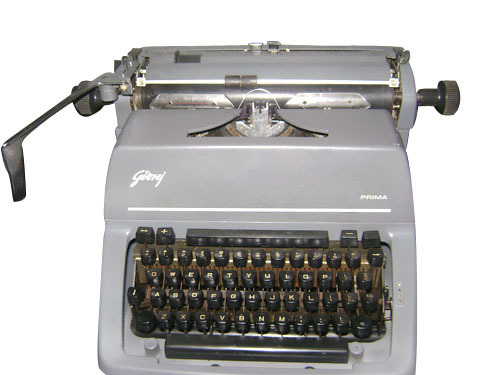
\includegraphics[width=\linewidth, height=5cm]{images/godrej-typewriter.jpg}
   \caption{Godrej typewriter}
\label{godrej}
\end{subfigure}%
\begin{subfigure}{.5\textwidth}
 \centering
 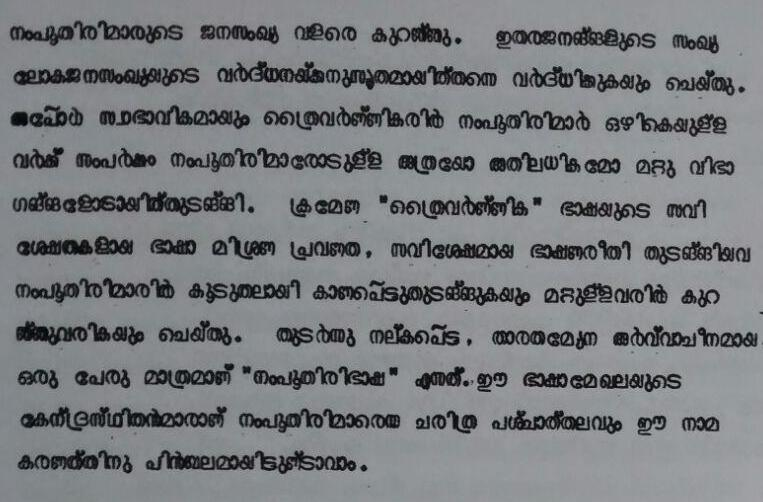
\includegraphics[width=\linewidth,height=5cm]{images/typewritertext4.jpg}
 \caption{Malayalam script typed by a typewriter}
 \label{typewritertext}
\end{subfigure}
\caption{A typewriter and its output}
\label{typewriter}
\end{figure}

\subsection{Implementation}

\paragraph{}
The print media switched to the reformed orthography in varying extends. The official prints of the government almost completely switched to the reformed style. Some publishers retained the graphemes for signed form of consonants but detatched the signed vowel forms. Publishers adopted a set of conjuncts as per their choice and splitted down the others using \textit{virama} sign. The new learners of the language learn the reformed orthographic style from the textbooks. But they continue to watch and learn the usage of traditional complex orthography widely seen in wall graffiti, poster designs and handwriting.



\section{Modern Evolution of the script}
\paragraph{}
The digitization of printing was yet another remarkable event. The pre-Unicode digital fonts in Malayalam were Malayalam letters mapped to the ASCII character space. Such fonts retained only a limited repertoire of conjuncts. Also the signed notations of vowels and consonants were detached from the base grapheme. Digital fonts before the unicode era embraced the reformed orthography more closely. The publishing industry largely depended on these fonts for decades.

\paragraph{}
At the same time, writing Malayalam in non-digital, non-printing contexts continue to use traditional orthography. Wall paintings, artistic lettering used in magazines, movie titles continued using it.

\paragraph{}
In 1998, an organization, named Rachana Aksharavedi was formed to bring back the orthography with the help of technology advancement. At that time, Malayalam was not encoded in Unicode. Rachana Aksharavedi developed a font named Rachana with about 1200 glyphs. Since there is no Unicode or opentype technology, it was a set of 6 fonts, each covering about 200 glyphs mapped to ASCII codepoints. A special editor known as Rachana Editor was required to automatically switch between these fonts and display Malayalam with data being English. This brave attempt was widely appreciated. A couple of years later Unicode encoding for Malayalam happened.

\paragraph{}
Rachana font was ported to Unicode. Parallel to that more unicode fonts emerged, notably AnjaliOldLipi. In 2006, Swathanthra Malayalam Computing(SMC), a free software developer community became active in Malayalam computing. Along with various language processing tools and technology improvements, SMC released a dozen of Malayalam fonts. Except one, all followed traditional orthography and embrased the opentype technology. These fonts became so popular among unicode Malayalam users and often preferred in operating systems than the default fonts. GNU/Linux systems came with these traditional orthography fonts by default. Schools and government institutions were using GNU/Linux systems because of Kerala government policy to use Free Software. The userbase of traditional orthography started to expand among digital Malayalam users. The IT education carriculum in schools also widely used these fonts.

\begin{wrapfigure}{L}{0.6\textwidth}
	\centering
	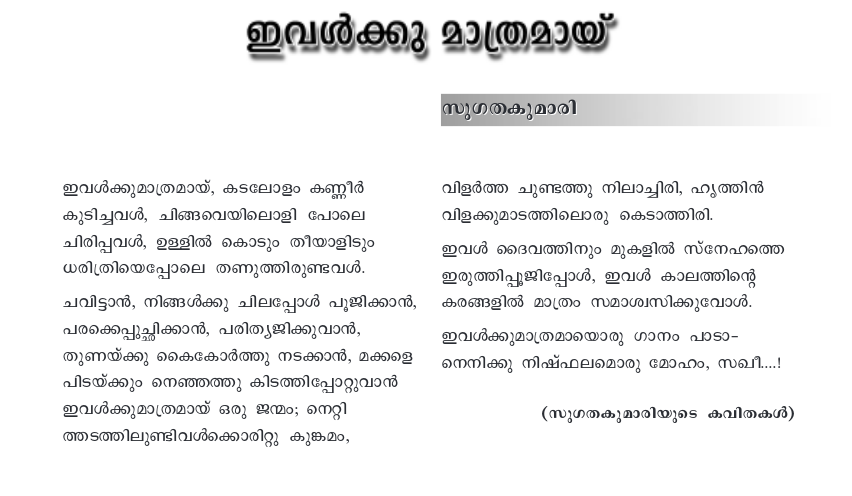
\includegraphics[width=0.5\textwidth]{images/2011-Malayalam-Textbook.png}
	\caption{Malayalam Textbook (2011). ASCII based new orthography in print}
	\label{textbook2011}
\end{wrapfigure}

\paragraph{}
But, the typesetting tools and softwares adapted to the ASCII based fonts became the default in the publishing industry. Even after the encoding of Malayalam in Unicode in \textit{2001}, the printing and publishing industry continued their practices. The Figure \ref{textbook2011}, shows the usage of ASCII based reformed orthography in print in 2011. This was largely due to lack of unicode and complex script rendering support in major typesetting systems like Adobe Indesign. But these typsetting systems started supporting complex scripts and now we are seeing a highly accelerated adoption of Unicode and traditional orthography in printing.

For example: Eureka, Samakalika malayalam


\begin{figure}[h!]
 \centering
  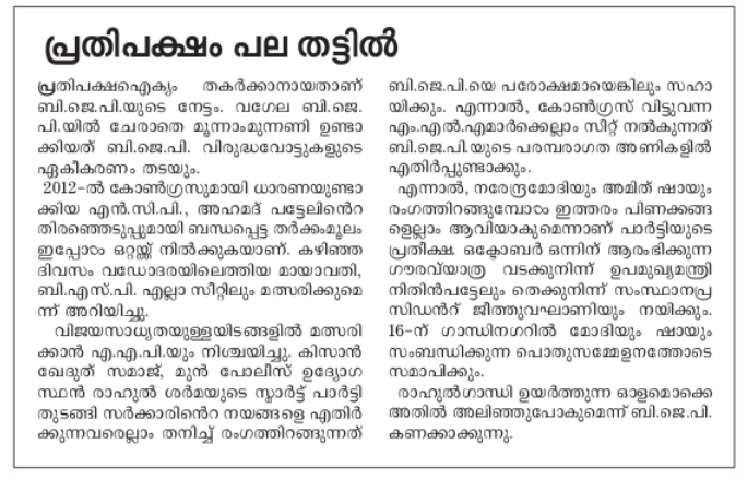
\includegraphics[width=1.0\textwidth]{images/2017-Mathrubhumi-newspaper.png}
   \caption{2017 Mathrubhumi news paper}
\end{figure}

\subsection{Unicode and Advanced Digital Typography}

\paragraph{}
With the advent of Unicode based digital typography, complex conjunct formations and their rendering were no more a technological challenge. With only the basic graphemes encoded in Unicode, any long sequence of consonants and signs could be mapped to a single conjunct grapheme in signed or unsigned form. Complex rendering rules of the script can easily be handled by modern rendering engines. With these technical advancements, fonts which could very well support the traditional orthographic scheme of the Malayalam script emerged. 

\paragraph{}
But the early years of Unicode based fonts and their rendering were never a cakewalk. \textit{Bug fixes in the rendering engine to fonts}. Adoption limited to digital usage, not to print.

\section{Modern Script Usage}
\paragraph{}

Lorem ipsum dolor sit amet, consectetur adipiscing elit, sed do eiusmod tempor incididunt ut labore et dolore magna aliqua. Ut enim ad minim veniam, quis nostrud exercitation ullamco laboris nisi ut aliquip ex ea commodo consequat. Duis aute irure dolor in reprehenderit in voluptate velit esse cillum dolore eu fugiat nulla pariatur. Excepteur sint occaecat cupidatat non proident, sunt in culpa qui officia deserunt mollit anim id est laborum.

\subsection{Internet}
\begin{figure}
 \centering
  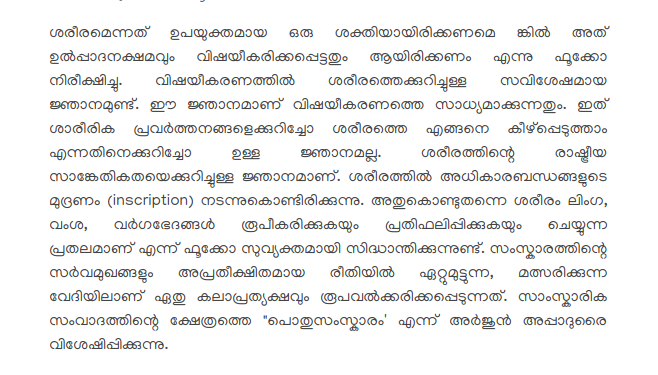
\includegraphics[width=1.0\textwidth]{images/Manjari-Body-Text.png}
   \caption{2017 Manjari font- a widely used unicode font}
\end{figure}


\textit{Eureka, Samakalika Malayalam}

\subsection{Government}
\paragraph{}

Lorem ipsum dolor sit amet, consectetur adipiscing elit, sed do eiusmod tempor incididunt ut labore et dolore magna aliqua. Ut enim ad minim veniam, quis nostrud exercitation ullamco laboris nisi ut aliquip ex ea commodo consequat. Duis aute irure dolor in reprehenderit in voluptate velit esse cillum dolore eu fugiat nulla pariatur. Excepteur sint occaecat cupidatat non proident, sunt in culpa qui officia deserunt mollit anim id est laborum.


\begin{figure}[h!]
 \centering
  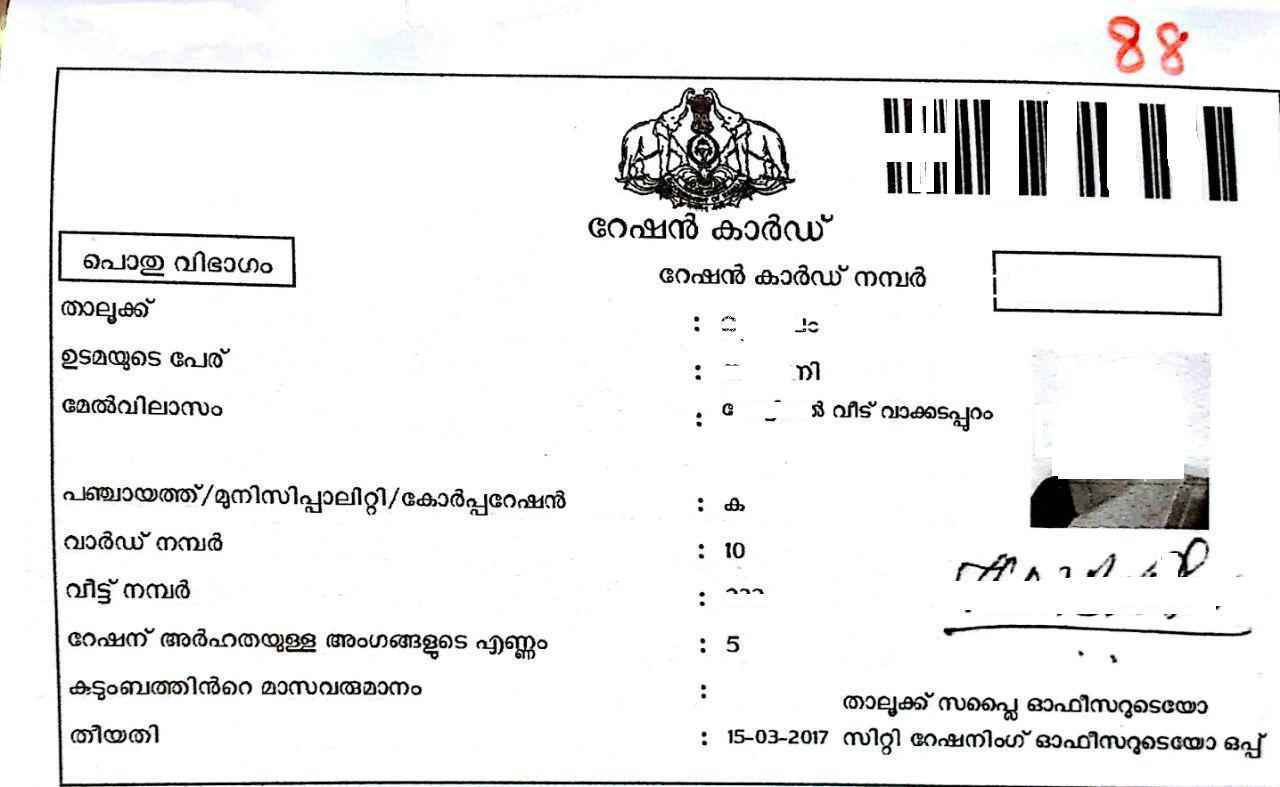
\includegraphics[width=1.0\textwidth]{images/2017-rationcard.jpg}
   \caption{2017 Ration card}
\end{figure}


\subsection{Posters and Memes}

\paragraph{}
Lorem ipsum dolor sit amet, consectetur adipiscing elit, sed do eiusmod tempor incididunt ut labore et dolore magna aliqua. Ut enim ad minim veniam, quis nostrud exercitation ullamco laboris nisi ut aliquip ex ea commodo consequat. Duis aute irure dolor in reprehenderit in voluptate velit esse cillum dolore eu fugiat nulla pariatur. Excepteur sint occaecat cupidatat non proident, sunt in culpa qui officia deserunt mollit anim id est laborum.


\begin{figure}[h!]
 \centering
  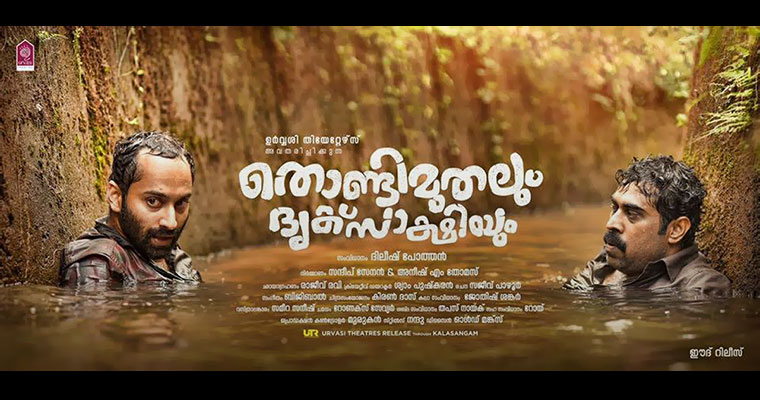
\includegraphics[width=1.0\textwidth]{images/2017-movieposter-Thondimuthal}
 \caption{A Malayalam movie poster from 2017. Uses traditional orthogrophy for title.}
\end{figure}
\paragraph{}
Lorem ipsum dolor sit amet, consectetur adipiscing elit, sed do eiusmod tempor incididunt ut labore et dolore magna aliqua. Ut enim ad minim veniam, quis nostrud exercitation ullamco laboris nisi ut aliquip ex ea commodo consequat. Duis aute irure dolor in reprehenderit in voluptate velit esse cillum dolore eu fugiat nulla pariatur. Excepteur sint occaecat cupidatat non proident, sunt in culpa qui officia deserunt mollit anim id est laborum.

\begin{figure}[h!]
 \centering
  
\includegraphics[width=1.0\textwidth]{images/2016-oru-muthashi-gadha}
 \caption{A Malayalam movie poster from 2016. Uses traditional orthogrophy for title.}
\end{figure}

\paragraph{}
Lorem ipsum dolor sit amet, consectetur adipiscing elit, sed do eiusmod tempor incididunt ut labore et dolore magna aliqua. Ut enim ad minim veniam, quis nostrud exercitation ullamco laboris nisi ut aliquip ex ea commodo consequat. Duis aute irure dolor in reprehenderit in voluptate velit esse cillum dolore eu fugiat nulla pariatur. Excepteur sint occaecat cupidatat non proident, sunt in culpa qui officia deserunt mollit anim id est laborum.


\begin{figure}[h!]
 \centering
  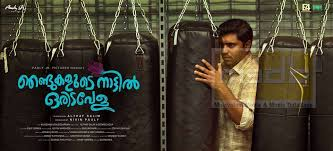
\includegraphics[width=1.0\textwidth]{images/2017-movieposter-njandukalude}
 \caption{A Malayalam movie poster from 2016. Uses traditional orthogrophy for title.}
\end{figure}

\section{Conclusion}

\paragraph{}
Technology played a crucial role in defining the orthography of Malayalam from printing to digital age. When technology like typewriters had limitations language also went through difficult reformation, but flourished again with the help digital technology. A single human generation is witnessing Malayalam's transition from traditional orthograhy to simplified orthography and then again to traditional orthography.

\begin{thebibliography}{9}
\bibitem{georgemathan} George Matthan, \textit{A Grammer of Malayalim in the Language itself }, CMS Press, 1863.
\bibitem{babucherian} Babu Cheriyan, \textit{Bebjamin Bailiyum Malayala Sahithyavum} {\manjari{(ബെഞ്ചമിൻ ബെയിലിയും മലയാള സാഹിത്യവും}) }, Mahatma Gandhi University, Kottayam, 2008
\bibitem{gupthannair} S. Gupthan Nair, \textit{Gadyam Pinnitta Vazhikal}{\manjari{ (ഗദ്യം പിന്നിട്ട വഴികൾ)} }, DC Books, Kottayam
\bibitem{1971go} Order by the Government of Kerala, India, G. O. (P) 37/71/Edn. , \textit{Malayalam Script- Adoption of New Script for Use-Orders Issued}, Dated 23 March, 1971.
•


\end{thebibliography}

\end{document}
